\section{加速度}
在描述物体的机械运动时,我们不仅要知道某一时刻物体在哪里(位移),向哪个方向运动的快慢(速度),而且也需要知道\CJKunderwave{物体速度变化的快慢},所以引入加速度.

\subsection{加速度}
\subsubsection{定义}
加速度定义为\CJKunderwave{速度的变化量}和\CJKunderwave{时间}的比值,如下
\begin{equation}
  a=\cfrac{\Delta v}{\Delta t} \label{eq:acceleration}
\end{equation}

\subsubsection{物理意义}
\CJKunderwave{加速度}是表征物体\CJKunderwave{速度变化快慢}的物理量.

\subsubsection{矢标性}
从定义上来看,速度的变化量$\Delta v$ 是矢量,时间 $\Delta t$ 是标量,所以加速度也是一个\CJKunderwave{矢量}.它的方向与\CJKunderwave{速度变化量}$\Delta v$ 的方向一致.
\subsubsection{单位}
从定义上来看,速度变化量的单位是$m/s$,时间的单位是$s$ ,所以加速度的单位是:\CJKunderwave{ 米每二次方秒},记作$m/s^2$

\subsection{瞬时加速度和平均加速度}
类比瞬时速度和平均速度,加速度也有瞬时加速度和平均加速度.

\subsubsection{瞬时加速度}
瞬时加速度用来描述某\CJKunderwave{一个时刻}速度变化的快慢.其定义如下:
\begin{equation}
a=\lim_{\Delta t \to 0} \cfrac{\Delta v}{\Delta t}
  \label{eq:instantaneous acceleration}
\end{equation}

\subsubsection{平均加速度}
平均加速度用来描述某\CJKunderwave{一段时间}内速度平均变化快慢.其定义如下:
\begin{equation}
\overline{a} =\cfrac{\Delta v }{\Delta t}
  \label{eq:average acceleration}
\end{equation}

\subsection{加速与减速的判断}

在具体的运动中,物体有可能加速也有可能减速,但是没有{\bf 减速度}一词.所有变速运动速度的变化量与
时间的比值都叫加速度,这只是一个名称而已.

如果物体运动的轨迹是直线,则称为直线运动,在直线运动中,如果 $v$ 与 $a$ 方向相同则加速,如果 $v$ 与 $a$ 的方向相反则减速.

如果物体运动的轨迹是曲线,则称为曲线运动,在曲线运动中,如果 $v$ 与 $a$ 的夹角是锐角则加速,如果 $v$ 与 $a$ 夹角为钝角则减速,如果 $v$ 与 $a$ 的夹角是直角,则速度大小不发生变化,只有速度的方向发生变化.

\subsection{注意事项}
在物理学中经常用比值定义法来定义物理量,这就好比用钱来定义钱包一样:\CJKunderwave{钱包是用来盛钱的包}.但是钱包和钱的多少没关系.所以加速度$a$ 和 $\Delta v$也没有关系,与$\Delta t$也没有关系,它\CJKunderwave{只取决于速度变化量和时间的比值}.

$\Delta$这个符号用来表示\CJKunderwave{一个末态的量减去一个初态的量},比如:$\Delta v =v_2 -v_1$,其中$v_1$是初始的速度,$v_2$是末速度.以后遇到的所有$\Delta$都具备此含义.

按上面的表述,则$\Delta t >0$是\CJKunderwave{永远成立}的.所以$a$与$\Delta v$的符号相同,因此说加速度的方向与速度变化量的方向一致.

\subsection{例题分析}
\begin{selection}
  1.一辆汽车正在公路上行驶,关于汽车的运动,下列说法正确的是
  A.汽车的速度改变量越大,加速度一定越大
  B.速度很大的汽车,其加速度可能很小,但不能为零
  C.某时刻汽车的速度为零,其加速度可能很大
  D.汽车加速度很大时,其速度一定很大

  a.C

  e.汽车的速度改变量越大,加速度不一定越大,因为加速度与速度改变量和时间间隔两个因素有关,选项A错误;速度很大的汽车,加速度可能很小,也可能为零,例如匀速直线运动的汽车,选项B 错误;汽车速度为零时,加速度可能很大,例如汽车刚启动时,选项C正确,D错误.

  2.由加速度的定义式$a=\cfrac{\Delta v}{\Delta t}$可知
  A.加速度$a$与速度的变化$\Delta v$ 成正比
  B.加速度$a$ 大小由速度变化$\Delta v$ 决定
  C.加速度$a$ 的方向与速度$v$ 的方向 相同
  D.加速度$a$ 的方向与$\Delta v$的方向相同

  a.D

  e.$a=\cfrac{\Delta v}{\Delta t} $ 是加速度的定义式,是比值定义法,不能说加速度与分子和分母单独有关,所以A,B 错误.由于$\Delta t>0$ 永远成立,所以 $a$ 的符号与$\Delta v$ 的正负号相同,一个矢量正负号表示方向,所以D 正确.

  3.某物体沿直线运动,其$v-t$ 图象如
  <:
  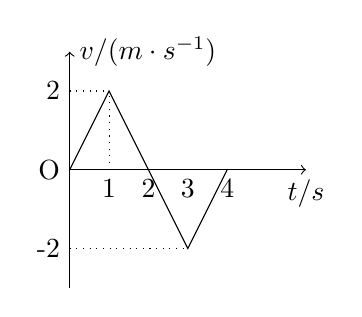
\begin{tikzpicture}
    \draw[->] (0,0)--(3,0) node [anchor=north ]{$t/s$};
    \draw[->] (0,-1.5)--(0,1.5) node [anchor=west]{$v/(m\cdot s^{-1})$};
    \draw (0,0) node [anchor=east] {O};
    \draw (0.5,0) node [anchor=north]{1};
    \draw (1,0) node [anchor=north]{2};
    \draw (1.5,0) node [anchor=north]{3};
    \draw (2,0) node [anchor=north]{4};
    \draw (0,0)--(0.5,1)--(1.5,-1)--(2,0);
    \draw [dotted](0,1)node [anchor=east]{2}--(0.5,1);
    \draw [dotted] (0.5,0)--(0.5,1);
    \draw [dotted](0,-1)node [anchor=east]{-2}--(1.5,-1);
  \end{tikzpicture}
  :>所示,下列说法正确的是
  A.第$1s$ 内和 第$2s$ 内物体的速度方向相反
  B.第$1s$ 内和第$2s$ 内物体的加速度方向相反
  C.第$3s$ 内物体的速度方向和加速度方向相反
  D.第$2s$ 末物体的加速度为零

  a.B

  e.速度的方向由纵坐标的正负表示,正号表示与正方向相同,负号表示与正方向相反.加速度的方向由$v-t$ 图象的斜率的正负表示,正号表示加速度沿正方向,负号表示加速度沿负方向.第$1s$ 内,第$2s$ 内纵坐标为正,速度均为正向,A错误;根据斜率的正负,第$1s$ 内加速度为正向,第$2s$ 内加速度为负方向,B正确;第$3s$ 内速度为负方向,加速度为负方向,C错误;第$2s$ 末物体的加速度为$-2m/s^2$,D错误.

\end{selection}
